\chapter{Biocrusts as climate-dependent regulators of erosion, water and nutrient cycling}
\label{chap:manuscript2} % Label for potential cross-referencing (start page)

\begin{center}
  \textbf{\Large Manuscript 2}
\end{center}

\vspace{0.1cm}

\begin{center}
  \textbf{\huge Biocrusts as climate-dependent regulators of erosion, water and nutrient cycling}
\end{center}

\vspace{0.2cm}

\begin{center}
  \textit{Geoderma}\\
  \textit{Submitted}
\end{center}
\vspace{0.1cm}

\begin{justify}
  Nicolás Riveras-Muñoz\textsuperscript{1}, Steffen Seitz\textsuperscript{1}, Corinna Gall\textsuperscript{1}, Victoria Rodríguez\textsuperscript{2}, Kristina Witzgall\textsuperscript{3}, Peter Kühn\textsuperscript{1}, Carsten W. Mueller\textsuperscript{4,5}, Rómulo Oses\textsuperscript{6}, Oscar Seguel\textsuperscript{7}, Dirk Wagner\textsuperscript{2,8}, and Thomas Scholten\textsuperscript{1}
\end{justify}

\vspace{0.2cm}

\begin{scriptsize}
  \begin{justify}
    \textsuperscript{1}University of T{\"u}bingen, Department of Geosciences, Soil Science and Geomorphology, R{\"u}melinstr. 19--23, 72070 T{\"u}bingen, Germany\\
    \textsuperscript{2}GFZ Helmholtz Centre for Geosciences, Section Geomicrobiology, Telegrafenberg, 14473 Potsdam, Germany\\
    \textsuperscript{3}Technical University of Munich, Soil Science, Emil-Ramann-Str. 2, 85354 Freising, Germany\\
    \textsuperscript{4}Technische Universit{\"a}t Berlin, Ernst-Reuter-Platz 1, 10587 Berlin, Germany\\
    \textsuperscript{5}Department of Geosciences and Natural Resource Management, University of Copenhagen, Copenhagen, Denmark\\
    \textsuperscript{6}Universidad de Atacama, Centro Regional de Investigaci{\'o}n y Desarrollo Sustentable de Atacama (CRIDESAT), Copayapu 485, Copiap{\'o}, Chile\\
    \textsuperscript{7}Universidad de Chile, Facultad de Ciencias Agron{\'o}micas, Av. Santa Rosa \#11315, La Pintana, 8820808 Santiago, Chile \\
    \textsuperscript{8}University of Potsdam, Institute of Geosciences, Karl-Liebknecht-Str. 24--25, 14476 Potsdam, Germany
  \end{justify}
\end{scriptsize}
  
\vspace{0.4cm}

\begin{flushleft}
  Submitted: March 17, 2025\\
\end{flushleft}

\cleardoublepage

\section*{Abstract} % Use \section* for unnumbered sections if needed

Biocrusts, complex communities of organisms, significantly alter surface and sub-surface processes, including water infiltration, and the cycling of carbon (C) and nitrogen (N). While their importance is recognized, studies across broad climatic gradients are scarce. We conducted rainfall simulation experiments at four sites along a \SI{910}{\kilo\meter} Chilean Coastal Range transect, representing coastal and inland semi-arid, mediterranean, and humid climates. We quantified overland flow, sediment discharge, and fluxes of C and N in percolating water, comparing paired biocrust-covered and bare soil surfaces. Our findings reveal that biocrusts, compared to bare soil, significantly increased cumulative infiltration rates across all climates, indicating enhanced saturated hydraulic conductivity. Biocrust presence reduced runoff by 73\% in humid climates and sediment flux by 80\% in inland semi-arid climates. On average, soil erosion was reduced by up to 69\%. Additionally, biocrusts significantly reduced C loss via erosion. Dissolved organic carbon and nitrogen fluxes were also strongly influenced by the presence of biocrusts. Overall, our study demonstrates that, though the presence of biocrust significantly reduced erosion, water and nutrient dynamic are strongly influence by its presence and the climates, showing that biocrusts act as climate-dependent regulators of crucial surface and sub-surface transport processes.

\section*{Keywords}

Biocrusts, Erosion, Infiltration, Climate gradient, Carbon, Nitrogen, Runoff

\section{Introduction}

Biological soil crusts (BSC) are formed by a close association between soil particles and various proportions of photoautotrophic organisms, such as cyanobacteria, algae, lichens, and bryophytes, along with heterotrophic organisms like bacteria, fungi, and archaea that live within or immediately above the top millimeters of the soil \citep{Weber2022}. They are a primary soil cover in arid environments, where the scarce availability of water limits the establishment of higher plants \citep{Ding2020,Weber2022}. However, biocrusts are also present in mesic environments without water limitation, where vascular plants and litter reduce their ability to compete \citep{Corbin2020,Gall2022a}. Nevertheless, biocrusts can be abundant in such areas when disturbance and the subsequent ecological succession provide favorable conditions for their establishment \citep{Budel2014,Gall2022a}.

Biocrust composition, growth, and survival depend on climatic factors such as temperature, moisture availability, and rainfall characteristics \citep{Belnap2003}. Moreover, climatic diversity shapes the morphological, chemical and physiological characteristics of the different biocrusts \citep{ConcostrinaZubiri2014}. In arid environments, biocrusts typically dominated by algae, cyanobacteria, and lichens, form smooth and flat surfaces that concentrate a large amount of microbial biomass and serve as nutrient sources within these ecosystems \citep{Weber2022}. In these settings, cyanobacteria can fix large amounts of nitrogen and produce reserve exopolysaccharides (EPS) that support other organisms \citep{RodriguezCaballero2018,Samolov2020}.

In addition, under humid conditions, biocrusts have a higher proportion of fungi and bryophytes, resulting in rough surfaces with a remarkable capacity to store capillary water, increased pore space in their structure and enhanced carbon fixation \citep{RiverasMunoz2022,Weber2022}. These changes in surface roughness affect the surface hydrology of the soil by modifying the residence time of water on the surface \citep{Kidron2022}. Changes in water residence time, in turn, affect the distribution of infiltration and runoff, alter surface redox conditions, modify soil erodibility, and regulate the release of solutes into water \citep{Kalnejais2010}. This emphasizes the ability of biocrusts to modify water and sediment fluxes. In particular, lichen-dominated dryland biocrusts can enhance surface runoff and reduce sediment yield by surface clogging and subsequently surface saturation, and runoff initiation \citep{Kidron2021}. They can also dramatically alter albedo, soil temperature dynamics and thus consequently the potential evapotranspiration \citep{Liu2020b,Rutherford2017,Whitney2017,Xiao2019}. Moss-dominated biocrusts with a rough morphology have a high water-holding potential and can decrease both runoff and sediment yield \citep{Juan2023,Seitz2017,Silva2019,Zeng2025}. Other effects of biocrusts that also include near-surface infiltration within the biocrust cover and its effect on percolation report enhanced infiltration and percolation in semi-arid ecosystems \citep{Chamizo2016} and reclaimed soils \citep{Gypser2016}, alteration rainwater flow in drylands \citep{Li2022}, and reduced infiltration while increasing erosion resistance in disturbed forests \citep{Szyja2023}. Moreover, comparative experimental studies focusing on soil water movement through different types of biocrust remain limited.

Along with their ability to modify water and sediment fluxes, biocrust communities significantly shape carbon (C) and nitrogen (N) cycles. Many researchers point biocrusts as one of the most important factors that initially influence soil organic carbon (SOC) in the uppermost soil horizon before higher plants appear (Belnap et al., 2007). Furthermore, \citet{Young2022} demonstrated that biocrusts facilitate the vertical movement of soluble carbon and nutrients from the surface to subsurface mineral soils, thereby enhancing overall carbon sequestration. The significance of biocrusts in the carbon cycle extends beyond their local role in building SOC \citep{Witzgall2024}, with these communities estimated to account for 7\% of total net carbon uptake and 50\% of terrestrial nitrogen fixation \citep{Elbert2012}. They further enhance C fixation through photosynthetic sequestration \citep{Belnap2016,Grote2010}. An increase in soil aggregate stability hinders C discharge by erosion \citep{RiverasMunoz2022,Xiao2022}, enhances soil fertility \citep{Kheirfam2017}, and fosters the establishment of other vascular and non-vascular organisms, further increasing C storage potential \citep{MolinaMontenegro2016}. In disturbed temperate forests, \citet{Gall2022b} found that mosses significantly influence the relocation of SOC and total N via soil erosion and percolation, further highlighting biocrusts’ impact on nutrient redistribution. Additionally, biocrusts play an active role in the N cycle as they are responsible for approximately 40 to 85\% of N fixation worldwide, mainly through the activity of cyanobacteria , enhances soil fertility \citep{Kheirfam2017}, and foster the establishment of other vascular and non-vascular organisms, further increasing C storage potential \citep{MolinaMontenegro2016}. Additionally, biocrusts play an active role in the N cycle as they are responsible for approximately 40 to 85\% of N fixation worldwide, mainly through the activity of cyanobacteria \citep{RodriguezCaballero2018b,Samolov2020}. As for C, biocrusts immobilize N by incorporating it into their biomass, thereby reducing losses by leaching or volatilization \citep{Nevins2020,Pan2021}. Furthermore, biocrusts can mineralize N from SOC, making it available to other organisms in the soil ecosystem \citep{Weber2015}.

All these properties of biocrusts impact soil erosion, a central process that shapes the Earth's surface \cite{Luetzenburg2020,Scholten2019}. Water-induced erosion occurs in humid and semi-humid regions \citep{Gholzom2012,Khaleghi2018} but also occurs in arid environments due to rare extreme rainfall events \citep{Hu2022}. Biocrusts not only influence infiltration and overland flow, but also form a physical barrier against erosive agents, partially absorbing the kinetic energy of running water and falling raindrops. A reduction of runoff by 25.6\% and sediment discharge by 75.5\% was observed when comparing runoff plots with biocrust cover below 10\% and above 50\% in early successional subtropical forests \citep{Seitz2017}. Similar effects of biocrusts on soil erosion have been reported in arid \citep{Bowker2018,Eldridge2021}, temperate (Gall et al., 2022a) and humid environments \citep{Guo2022,Zhao2014}. Another process of land surface stabilisation by biocrusts is the formation of aggregates from organic and mineral particles through the secretion of bacterial metabolites such as exo- and lipopolysaccharides \citep{Costa2018,Tourney2014,Xiao2022}. Further, the trapping of soil particles within the structures of biocrusts helps prevent soil erosion \citep{RiverasMunoz2022,Rodriguez2024,Xiao2022}.

Biocrusts are increasingly observed and described outside their classical dryland habitats—hyper-arid, arid, semi-arid, and dry sub-humid habitats \citep{Gall2022a,Weber2022}. Furthermore, investigations into climate variability have covered multiple scales. For example, \citet{MunozMartin2019} studied cyanobacterial biocrust diversity along an aridity gradient in Mediterranean semi-arid soils and found that temperature and precipitation determine biocrust composition, with a greater prevalence of extremotolerant in harsher climates. Regarding topography, \citet{CastilloMonroy2016} reported that species composition and richness of biocrusts increase with elevation in tropical shrublands. Additionally, \citet{Ding2020} observed that, on smaller spatial scales in Australia, microsite differences correlate with an increase in biocrust cover as aridity rises, while \citet{RiverasMunoz2022} demonstrated that soil aggregate stabilization by biocrust improved from arid to humid climates in Chile. Both studies reveal that the dominant structuring mechanisms of biocrusts shift with climate: under dry conditions, biocrusts stabilize the soil surface through exopolysaccharide production that promotes aggregate formation and structural stability, evidenced by the development of water-stable aggregates; whereas under humid conditions, biocrust structures further entangle and stabilize the soil surface, resulting in a more defined crust \citep{RiverasMunoz2022}. Although studies investigating the role of biocrusts in regulating water, sediment, and C and N fluxes in different climates are limited, the interactions and feedback mechanisms between the underlying processes are not yet fully understood.

To enhance our understanding of the interrelation between climate and the multifunctional roles of biocrusts in regulating water, sediment, and matter fluxes at the soil surface and within the topsoil, we conducted a field experiment comparing land surfaces with and without biocrusts. We quantified changes in C and N fluxes, both in particulate and water-dissolved forms influenced by the presence of biocrusts. Additionally, we examined how biocrusts modulated the interactions between water, sediment, and nutrient fluxes along a gradient ranging from arid to humid climates. We introduced a new measuring device capable of simultaneously sampling runoff, sediment and seepage flow in an undisturbed soil monolith during simulated rainfall events. This study focused on four sites within the Coastal Mountain Range of Chile, representing a climate gradient that includes coastal and inland semi-arid, Mediterranean and humid climates. All study sites (Figure \ref{fig:M2-F1}) have a comparable topography and almost the same parent materials. Our experimental approach utilizing undisturbed soil monoliths subjected to standardized rainfall simulations allows us to assess biocrusts' effects on various fluxes. Our main hypotheses are that (i) biocrusts modify runoff, sediment discharge and percolation flow, including liquid and solid C and N fluxes and reduce soil erosion irrespective of climatic conditions, but (ii) feedbacks between overland flow, percolation flow, sediment and liquid and solid C and N fluxes are climate specific.

\section{Materials and methods}
\subsection{Study sites}

Rainfall simulation experiments were conducted on four study sites over a \SI{910}{\kilo\meter}gradient from \ang{29} to \ang{38} S in the Chilean Coastal Range (Figures \ref{fig:M2-F1} and \ref{fig:M2-F2}). The study sites consist of coastal semi-arid shrubland (Santa Gracia Natural Reserve, henceforth SG), inland semi-arid shrubland (Quebrada de Talca Private Reserve, henceforth QdT), mediterranean forest (La Campana National Park, henceforth LC) and highland temperate rainforest (Nahuelbuta National Park, henceforth NA) \citep{Canessa2022}. All study sites have comparable topography, granitic parent material, and no glacial and volcanic influence \citep{Bernhard2018}. The study sites are located within protected natural areas, with limited human influence compared to the surrounding areas. Nonetheless, cattle occasionally enter these locations, and goats, mules, and donkeys have been reported to SG \citep{Armesto2007}.

\begin{figure}[H]
	\centering
	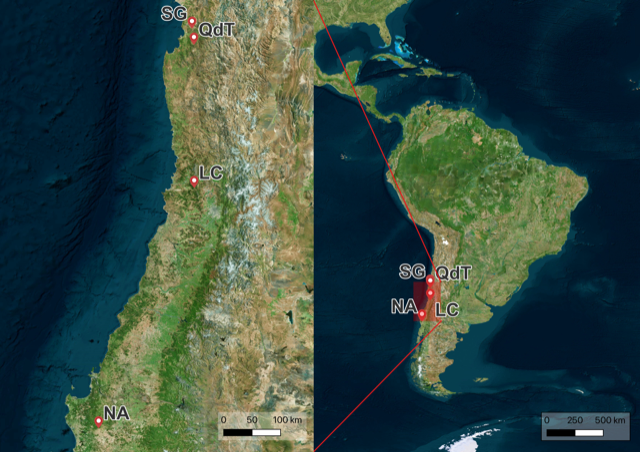
\includegraphics[width=1\textwidth]{img/M2-Figure_1.png}
	\caption{Location of the four study sites (left) relative to South America (right). From north to south: Santa Gracia (SG), Quebrada de Talca (QdT), La Campana (LC), and Nahuelbuta (NA). Bing Satellite (obtained through QuickMapServices QGIS plugin), Map data $©$2022 Microsoft.}
	\label{fig:M2-F1}
\end{figure}

\FloatBarrier

\begin{figure}[H]
	\centering
	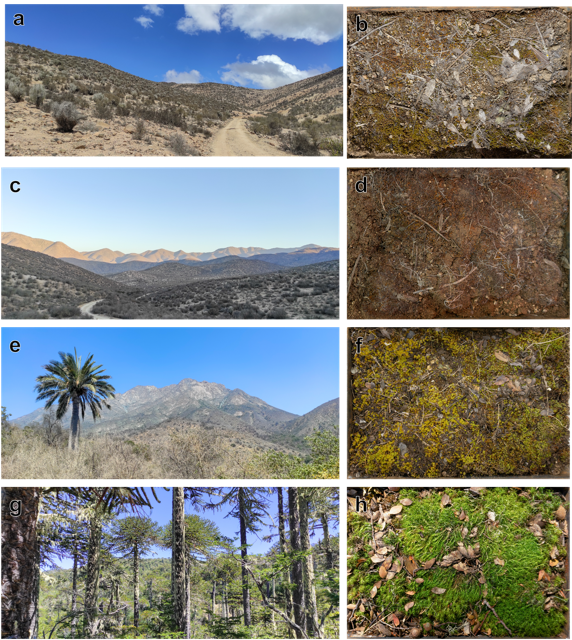
\includegraphics[width=1\textwidth]{img/M2-Figure_2.png}
	\caption{Overview of the study sites, showing the general landscape of Santa Gracia (SG) (a), Quebrada de Talca (QdT) (c), La Campana (LC) (e), and Nahuelbuta (NA) (g). Corresponding biocrusts are illustrated in photographs (b, d, f, h). Notable biocrust features include lichen-dominated communities in SG and moss-dominated communities in NA.}
	\label{fig:M2-F2}
\end{figure}

\FloatBarrier

Mean annual temperature (MAT) decrease and mean annual precipitation (MAP) increase from north to south (SG: \SI{13.7}{\degreeCelsius}, \SI{66}{\milli\metre\,\year^{-1}}; QdT: \SI{14.3}{\degreeCelsius}, \SI{109}{\milli\metre\,\year^{-1}}; LC: \SI{14.1}{\degreeCelsius}, \SI{367}{\milli\metre\,\year^{-1}}; NA: \SI{6.6}{\degreeCelsius}, \SI{1469}{\milli\metre\,\year^{-1}}). Despite the close distance between SG and QdT, \citet{Santibnez2017} classified both sites as different climatic districts. SG is climatically influenced mainly by the short distance to the coast, while QdT represents an inland climate with an increase of 4.4\% in MAT and 65.2\% in MAP compared to SG. Rainfall is concentrated in winter from May to August \citep{Bernhard2018,Canessa2020}. Paleoclimate modelling studies \citep{Mutz2018} indicate that these climate patterns have persisted since the late Pliocene. Thus, the study sites represent the constant long-term impact of climate on soil formation \citep{Ewing2006}. \citet{Bernhard2018} classified the soils according to the WRB system (2017) as Cambisols for SG, QdT, and LC and Umbrisols in NA according to a significant increase in topsoil SOC from north to south along the climate gradient. Soil baseline was characterized by \citet{RiverasMunoz2022} using topsoil samples (\SIrange[range-phrase=--,range-units=single]{0}{5}{\centi\meter}). Particle size distribution was determined for 7 fractions according to \citet{Kohn1929}, combining sieving of fractions $>$\SI{20}{\micro\meter} and pipetting of fractions $<$\SI{20}{\micro\meter}. Soil texture was interpreted according to the World Reference Base (WRB) soil classification system \citep{Jahn2006}.

The taxonomical composition of mosses and lichens present in the biocrust (Figure \ref{fig:M2-F2}) was described more extensively in \citep{RiverasMunoz2022}. At the dry end of the gradient, SG was dominated by lichens, and QdT exhibited a similar composition; in contrast, LC was mainly composed of mosses, while NA included mosses, liverworts and fungi.

\subsection{Rainfall simulation experiment}

At the research sites, one-square-meter plots were established for the actual rainfall simulation experiments. Each plot was located at top slope with a south-facing orientation. The setups considered the presence of site-typical biocrust communities, similar slope and aspect, and a lack of anthropogenic disturbance and ensured that the distance between each plot did not exceed 30 meters. Rainfall simulation was designed as a factorial, completely randomized experiment with eight treatments (four sites, each with and without biocrust). Five field replicates and three soil samples as technical replicates were taken, resulting in a sample size of n = 120 rainfall simulations.

Infiltration boxes (Figure \ref{fig:M2-F3}) were developed as part of a rainfall simulation experiment to measure runoff and percolation flow, including their matter content. Undisturbed soil samples were collected using cutting frames (\SI{20}{\centi\metre} $\times$ \SI{30}{\centi\metre} $\times$ \SI{7}{\centi\metre}, Figure \ref{fig:M2-F3}a), carefully installed with minimal surface and subsurface disturbances (Figure \ref{fig:M2-F3}c, Seitz (2015)). Cutting frames are made from \SI{1}{\milli\meter} metal plates, sharpened in the bottom sides, and include an upper border to transfer the strength to them without direct contact with the soil and a lower one to stop the frame from burying beyond the desired height of the sample (Figure \ref{fig:M2-F3}a). Subsequently, the cutting frames were excavated around, and a metal plate was inserted underneath it (Figure \ref{fig:M2-F3}d). The cutting frames with the soil samples were covered with metal plates, wrapped in plastic foil, and carefully transported to a flat area with water available. Then, the wrappings were removed, and the frames with the soil samples were stacked on a permeable metal plate and placed inside the soil erosion flux box (Figure \ref{fig:M2-F3}a) designed as steel containers with a triangular surface runoff gutter and an outlet at the bottom to capture the percolation flow (Figure \ref{fig:M2-F3}a). Soil depth within the boxes is \SI{7}{\centi\meter}. In the case of the presence of small plants, they were cut flush with the surface using a scissor and paying attention to not pull them and avoid surface disturbances. The water content of each sample was measured by a TDR probe (Delta-T Devices Ltd. Cambridge, UK) when sampling, using the average of 3 measurements directly next to the sampling area. Perpendicular photographs were taken on each sample with a digital camera (Sony ILCE-6000 equipped with a lens SELP1650, Tokyo, Japan) and processed with the grid quadrat method overlying a digital grid of 100 subdivisions and separating biocrusts by visual inspection \citep{Belnap2001} to assess the biocrust ground cover.

\begin{figure}[H]
	\centering
	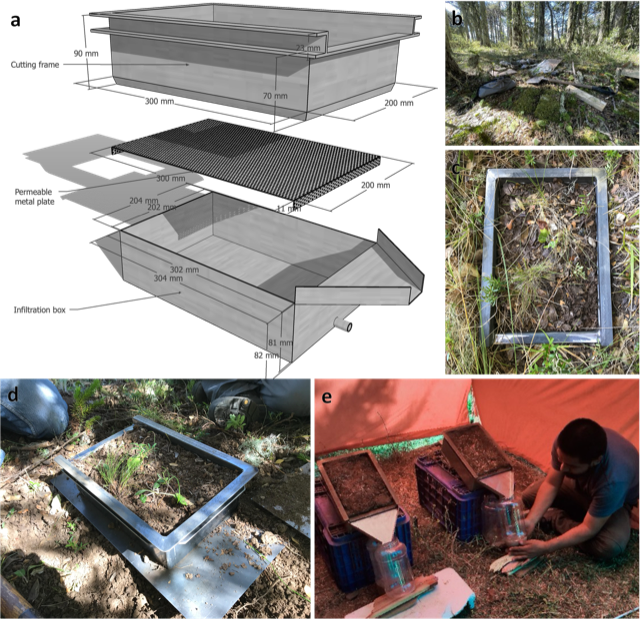
\includegraphics[width=1\textwidth]{img/M2-Figure_3.png}
	\caption{Construction diagram of the soil erosion flux box used in the experiment (a), general view of a plot with the presence of biocrust prior to sampling (b). (c, d) shows an installed cutting frame and the cleared and prepared soil. (e) demonstrates the setting for rainfall simulations at the Nahuelbuta (NA) study site.}
	\label{fig:M2-F3}
\end{figure}

\FloatBarrier

Rainfall simulations were conducted near the sampling site with the Tübingen rainfall simulator \citep{Iserloh2013,Seitz2015}, equipped with a Lechler 460.788.30 nozzle and adjusted to a falling height of \SI{3.5}{\meter}. The stack with the sample was placed inside the rainfall simulator and set to a \ang{10} slope (Figure \ref{fig:M2-F3}e). A rainfall event was simulated using an intensity of \SI{45}{\milli\metre\per\hour} sustained over a 30‐minute period. According to regional intensity-duration-frequency analyses for central Chile \citep{PizarroTapia2020}, such an intensity falls within the extreme rainfall category, well above the heavy precipitation threshold even for relatively wet climates. This extreme intensity was selected to exceed the soil infiltration capacities and reliably generate surface runoff at all study sites. In particular, the four sites represent a pronounced climatic gradient, ensuring that the simulated storm event is sufficiently intense to produce runoff under the diverse hydrological conditions encountered across these regions. The time to start runoff and percolation generation was recorded with a timer. Sediment-water samples were collected in bottles at the runoff gutter and percolation valve. The volume of water was registered with a graduated beaker. The samples were left to sedimentation by gravity, and a water sample was extracted from the supernatant using a siphon and frozen at \SI{-4}{degreeCelsius}. The remaining sample was dried in an oven at \SI{105}{degreeCelsius} until no water was observed and then for 48 hours. The weight of the sediment was measured using a balance, and the total C and N content of the sediment was subsequently analyzed. The sediment load was calculated by dividing the sediment amount by the water volume. The nutrient load on sediments was measured using an elemental analyzer (Vario EL III, Elementar Analysensysteme GmbH, Hanau, Germany). The water samples were filtered to \SI{0.45}{\micro\meter} and analyzed for DOC and DON using a Multi N/C 2100 S from Analytik Jena (Jena, Germany).

\subsection{Statistical analysis}

The experiment was designed as a factorial combination of site (4 levels) and biocrust (2 levels). Differences in the properties analyzed were proven by ANCOVA, using the soil baseline variables clay, silt, sand, C\textsubscript{T}, and N\textsubscript{T} as covariates. When covariates were not significant, analyzes continued using ANOVA. ANCOVA and ANOVA were implemented in R using the package stats 4.2.1 \citep{RCoreTeam2022}. In case normality or homoscedasticity were not accomplished, automatic data transformation was applied using the package bestNormalize 1.8.3 \citep{Peterson2021,Peterson2020}. We evaluated the normal distribution of the data using Shapiro-Wilk's Normality Test ($p> 0.05$) implemented in R stats 4.2.1 \citep{RCoreTeam2022} and homoscedasticity by Levene's Test ($p<0.05$) implemented in the car 3.1-0 package \citep{Fox2018}. The individual significance of treatments was assessed by the Dunn-Šidák correction implemented in the package multcomp 1.4-20 \citep{Hothorn2008}.

\section{Results}
\subsection{Surface runoff, percolating water fluxes, and their interrelation with biocrust cover along different climatic conditions}

Our findings reveal that biocrusts play a critical role in modulating associated with erosion, runoff, and percolation across varying climatic conditions (Table \ref{tab:M2-runoff_fluxes} and \ref{tab:M2-percolation_fluxes}). Overall, the time required to start runoff was significantly longer in NA, with the shortest time observed in the coastal arid site, SG. Biocrusts significantly delayed runoff initiation by 97.7\%, mainly due to increased surface roughness. This delay was more pronounced in NA, where the combination of enhanced roughness and high infiltration capacity extended the time for runoff initiation by three to four times. However, these effects did not extend to the subsoil, as biocrust had no measurable impact on the time needed for percolation to start.

The total runoff volume was significantly higher in SG compared to the other sites. Biocrust contributed to a significant reduction of the runoff volume, averaging a 28.0\% reduction, corresponding to a significant 50.0\% reduction in percolation. Regarding site-specific effects, biocrusts significantly reduced the runoff volume by 72.4\% in NA. Contrarily, a contrasting trend in LC was observed, with a 36.4\% increase in runoff volume associated with the biocrust presence.

The climatic gradient significantly influenced the total sediment transported by runoff, decreasing sediment mobilization as humidity increased. Biocrusts were pivotal in reducing sediment transport via runoff, resulting in an overall decrease of 69.9\%. However, this reduction in runoff-associated sediment transport was accompanied by a 28.3\% increase in the sediment mobilization via percolation. The interaction between the study site and biocrust presence showed significant sediment reductions across the northern sites, with NA exhibiting a similar trend, albeit without statistical significance.

The sediment load in the runoff, measured as sediment concentration in water, was significantly reduced by an average of 60.9\% in the presence of biocrust. In contrast, sediment concentration in percolation increased significantly by 58.3\%, highlighting a shift in sediment dynamics influenced by biocrust interactions across the study sites.

  % --- Table 1 Code (Runoff Fluxes) ---
\begin{table}[htbp] % Changed from sidewaystable
    \centering
    \footnotesize % Reduced font size for the table
    \sisetup{separate-uncertainty = true, table-align-uncertainty = true}
    \begin{threeparttable}
      \caption{Surface runoff fluxes on the study sites (SG: Santa Gracia, QdT: Quebrada de Talca, LC: La Campana, NA: Nahuelbuta) with (+) and without (-) biocrust (BSC) cover. Values correspond to mean $\pm$ standard deviation (SD) of five field replicates. A letter-based display of Šidák correction accompanies surface runoff parameters\tnote{a}, and the significance of the studied factors is shown as a p-value and list of covariates (C\textsubscript{T}, N\textsubscript{T}: total carbon and nitrogen content). Different letters indicate statistically significant different values based on our data, ns: non-significant.}
      \label{tab:M2-runoff_fluxes}
      \setlength{\tabcolsep}{3pt} % Reduced further slightly
  
      \begin{tabular}{@{} l l S[table-format=3.1, table-figures-uncertainty=4] @{\,} c
                             S[table-format=2.0, table-figures-uncertainty=2] @{\,} c
                             S[table-format=3.0, table-figures-uncertainty=3] @{\,} c
                             S[table-format=2.1, table-figures-uncertainty=3] @{\,} c
                          @{}}
        \toprule
        \multicolumn{2}{@{}l}{\multirow{3}{*}{\textbf{Factor}}} &
        {\makecell{\textbf{Time to}\\\textbf{start}\\\textbf{runoff}}} & & % Added line break for width
        {\makecell{\textbf{Runoff}}} & &
        {\makecell{\textbf{Sediment}\\\textbf{in runoff}}} & & % Added line break
        {\makecell{\textbf{Sediment}\\\textbf{load of}\\\textbf{runoff}}} & \\ % Added line breaks
        \cmidrule(lr){3-3} \cmidrule(lr){5-5} \cmidrule(lr){7-7} \cmidrule(lr){9-9}
        \multicolumn{2}{@{}l}{} & {[\si{\second}]} & & {[\si{L.h^{-1}}]} & & {[\si{g.m^{-2}.h^{-1}}]} & & {[\si{g.L^{-1}.m^{-2}}]} & \\
        \midrule
        \multicolumn{2}{@{}l}{\textbf{Mean} $\pm$ \textbf{SD}} & & & & & & & & \\
        & Site \quad SG  & 65.1 \pm 20.7 & {(a)}  & 49 \pm 18 & {(b)}  & 617 \pm 473 & {(c)}  & 12.1 \pm 7.9 & {(a)} \\
        & \phantom{Site \quad} QdT & 78.7 \pm 30.4 & {(a)}  & 40 \pm 16 & {(a)}  & 398 \pm 459 & {(b)}  & 9.6 \pm 9.6 & {(a)} \\
        & \phantom{Site \quad} LC  & 83.5 \pm 56.0 & {(a)}  & 39 \pm 22 & {(a)}  & 241 \pm 293 & {(b)}  & 7.3 \pm 8.8 & {(a)} \\
        & \phantom{Site \quad} NA  & 236.7 \pm 273.0 & {(b)} & 44 \pm 43 & {(a)}  & 28 \pm 44 & {(a)}   & 3.0 \pm 14.0 & {(a)} \\
        \addlinespace
        & Biocrust \quad BSC+ & 154.0 \pm 211.5 & {(b)} & 36 \pm 21 & {(a)}  & 149 \pm 222 & {(a)}  & 4.5 \pm 10.4 & {(a)} \\
        & \phantom{Biocrust \quad} BSC-- & 77.9 \pm 33.8 & {(a)}  & 50 \pm 31 & {(b)}  & 495 \pm 492 & {(b)}  & 11.5 \pm 10.0 & {(b)} \\
        \midrule
        \multicolumn{2}{@{}l}{\textbf{Site*Biocrust}} & & & & & & & & \\
        & SG \quad BSC+  & 62.7 \pm 21.2 & {(ab)}  & 44 \pm 16 & {(ab)} & 340 \pm 340 & {(bc)} & 7.5 \pm 5.7 & {(abc)} \\
        & SG \quad BSC--  & 67.5 \pm 20.6 & {(ab)}  & 54 \pm 18 & {(ab)} & 873 \pm 456 & {(d)}  & 16.7 \pm 7.1 & {(de)} \\
        & QdT \quad BSC+ & 87.3 \pm 37.5 & {(ab)}  & 38 \pm 15 & {(ab)} & 131 \pm 96 & {(ab)}  & 3.3 \pm 2.0 & {(abd)} \\
        & QdT \quad BSC-- & 70.1 \pm 18.7 & {(ab)}  & 42 \pm 18 & {(ab)} & 665 \pm 524 & {(cd)} & 15.8 \pm 10.2 & {(ce)} \\
        & LC \quad BSC+  & 85.8 \pm 67.1 & {(ab)}  & 45 \pm 20 & {(ab)} & 87 \pm 94 & {(a)}   & 2.1 \pm 1.9 & {(a)} \\
        & LC \quad BSC--  & 81.2 \pm 44.6 & {(ab)}  & 33 \pm 23 & {(ab)} & 395 \pm 344 & {(bc)} & 12.6 \pm 9.9 & {(bcde)} \\
        & NA \quad BSC+  & 380.4 \pm 329.5 & {(b)} & 19 \pm 23 & {(a)}  & 16 \pm 49 & {(a)}   & 5.2 \pm 19.9 & {(abcde)} \\
        & NA \quad BSC--  & 93.0 \pm 40.2 & {(a)}   & 69 \pm 45 & {(b)}  & 40 \pm 36 & {(a)}   & 0.9 \pm 1.2 & {(abcde)} \\
        \midrule
        \multicolumn{2}{@{}l}{\textbf{Significance} ($p$-value)} & & & & & & & & \\
        & Site         & \num{1.03e-05} & \tnote{*} & \num{0.0304} & \tnote{*} & \num{2.21e-14} & \tnote{*} & \num{1.93e-09} & \tnote{*} \\
        & Biocrust     & \num{0.01452} & \tnote{*} & \num{0.0034} & \tnote{*} & \num{4.37e-11} & \tnote{*} & \num{7.57e-10} & \tnote{*} \\
        & Site*Biocrust& \num{0.0166}  & \tnote{*} & \num{1.83e-05} & \tnote{*} & \num{0.00129}  & \tnote{*} & \num{0.000177} & \tnote{*} \\
        \midrule
        \multicolumn{2}{@{}l}{\textbf{Covariates}} &
        \multicolumn{2}{@{}l}{clay + C\textsubscript{T}} &
        \multicolumn{2}{@{}l}{silt + sand + N\textsubscript{T}} &
        \multicolumn{2}{@{}l}{} &
        \multicolumn{2}{@{}l}{\makecell[tl]{clay + sand + C\textsubscript{T} + \\ soil water content}} \\
        \bottomrule
      \end{tabular}
      \begin{tablenotes}[para,flushleft]
        \item[a] Letters indicate significant differences between means according to post-hoc tests with Šidák correction for multiple comparisons. Levels not sharing any letter are significantly different (p < 0.05).
        \item[*] Statistically significant effect (p < 0.05).
        \item[SD] Standard Deviation.
        \item[C\textsubscript{T}] Total Carbon content.
        \item[N\textsubscript{T}] Total Nitrogen content.
      \end{tablenotes}
    \end{threeparttable}
  \end{table}
  
% --- Table 2 Code (Percolation Fluxes) ---
  \begin{table}[htbp] % Changed from sidewaystable
    \centering
    \footnotesize % Reduced font size for the table
    \sisetup{separate-uncertainty = true, table-align-uncertainty = true}
    \begin{threeparttable}
      \caption{Percolating water fluxes on the study sites (SG: Santa Gracia, QdT: Quebrada de Talca, LC: La Campana, NA: Nahuelbuta) with (+) and without (-) biocrust (BSC) cover. Values correspond to mean $\pm$ standard deviation (SD) of five field replicates. A letter-based display of Šidák correction accompanies surface runoff parameters\tnote{a}, and the significance of the studied factor is shown as a p-value and list of covariates (C\textsubscript{T}, N\textsubscript{T}: total carbon and nitrogen content). Different letters indicate statistically significant different values based on our data, ns: non-significant.}
      \label{tab:M2-percolation_fluxes}
      \setlength{\tabcolsep}{3pt} % Reduced further slightly
  
      \begin{tabular}{@{} l l S[table-format=3.2, table-figures-uncertainty=4] @{\,} c
                             S[table-format=2.2, table-figures-uncertainty=3] @{\,} c
                             S[table-format=2.0, table-figures-uncertainty=2] @{\,} c
                             S[table-format=1.1, table-figures-uncertainty=3] @{\,} c
                          @{}}
        \toprule
        \multicolumn{2}{@{}l}{\multirow{3}{*}{\textbf{Factor}}} &
        {\makecell{\textbf{Time to start}\\\textbf{percolation}\\\textbf{flow}}} & & % Added line break
        {\makecell{\textbf{Percolation}}} & &
        {\makecell{\textbf{Sediments in}\\\textbf{percolation}\\\textbf{flow}}} & & % Added line breaks
        {\makecell{\textbf{Sediment load}\\\textbf{in percolation}}} & \\ % Added line break
        \cmidrule(lr){3-3} \cmidrule(lr){5-5} \cmidrule(lr){7-7} \cmidrule(lr){9-9}
        \multicolumn{2}{@{}l}{} & {[\si{\second}]} & & {[\si{L.h^{-1}}]} & & {[\si{g.m^{-2}.h^{-1}}]} & & {[\si{g.L^{-1}.m^{-2}}]} & \\
        \midrule
        \multicolumn{2}{@{}l}{\textbf{Mean} $\pm$ \textbf{SD}} & & & & & & & & \\
        & Site \quad SG  & 223 \pm 190   &        & 18.0 \pm 14 & {(a)}  & 19 \pm 34 &        & 4.2 \pm 19.7 &       \\
        & \phantom{Site \quad} QdT & 175 \pm 94.5  &        & 22.8 \pm 15 & {(a)}  & 7 \pm 10  &        & 0.2 \pm 0.3  &       \\
        & \phantom{Site \quad} LC  & 234 \pm 183   &        & 22.4 \pm 13 & {(a)}  & 13 \pm 15 &        & 0.5 \pm 0.5  &       \\
        & \phantom{Site \quad} NA  & 145 \pm 169   &        & 65.0 \pm 39 & {(b)}  & 23 \pm 25 &        & 0.4 \pm 0.4  &       \\
        \addlinespace
        & Biocrust \quad BSC+ & 171 \pm 133   &        & 42.6 \pm 34 & {(b)}  & 19 \pm 22 & {(b)}  & 0.5 \pm 0.5  &       \\
        & \phantom{Biocrust \quad} BSC- & 218 \pm 190   &        & 21.5 \pm 21 & {(a)}  & 12 \pm 24 & {(a)}  & 2.1 \pm 13.7 &       \\
        \midrule
        \multicolumn{2}{@{}l}{\textbf{Site*Biocrust}} & & & & & & & & \\
        & SG \quad BSC+  & 202 \pm 103   &        & 24.8 \pm 15 & {(ab)} & 19 \pm 18 &        & 0.7 \pm 0.5  &       \\
        & SG \quad BSC-  & 244 \pm 251   &        & 11.1 \pm 10 & {(a)}  & 18 \pm 46 &        & 7.5 \pm 27.5 &       \\
        & QdT \quad BSC+ & 148 \pm 63.9  &        & 30.5 \pm 13 & {(b)}  & 9 \pm 13  &        & 0.3 \pm 0.3  &       \\
        & QdT \quad BSC- & 202 \pm 113   &        & 15.1 \pm 13 & {(ab)} & 5 \pm 6   &        & 0.2 \pm 0.2  &       \\
        & LC \quad BSC+  & 226 \pm 223   &        & 23.5 \pm 14 & {(ab)} & 17 \pm 19 &        & 0.6 \pm 0.5  &       \\
        & LC \quad BSC-  & 241 \pm 139   &        & 21.3 \pm 14 & {(ab)} & 9 \pm 9   &        & 0.4 \pm 0.3  &       \\
        & NA \quad BSC+  & 107 \pm 35.6  &        & 91.5 \pm 28 & {(c)}  & 30 \pm 32 &        & 0.4 \pm 0.4  &       \\
        & NA \quad BSC-  & 183 \pm 234   &        & 38.5 \pm 30 & {(b)}  & 16 \pm 15 &        & 0.4 \pm 0.3  &       \\
        \midrule
        \multicolumn{2}{@{}l}{\textbf{Significance} ($p$-value)} & & & & & & & & \\
        & Site         & \multicolumn{2}{c}{(ns)} & \num{1.78e-12} & \tnote{*} & \multicolumn{2}{c}{(ns)} & \multicolumn{2}{c}{(ns)} \\
        & Biocrust     & \multicolumn{2}{c}{(ns)} & \num{8.11e-08} & \tnote{*} & \num{0.00946} & \tnote{*} & \multicolumn{2}{c}{(ns)} \\
        & Site*Biocrust& \multicolumn{2}{c}{(ns)} & \num{0.00164} & \tnote{*} & \multicolumn{2}{c}{(ns)} & \multicolumn{2}{c}{(ns)} \\
        \midrule
        \multicolumn{2}{@{}l}{\textbf{Covariates}} &
        \multicolumn{2}{@{}l}{clay} &
        \multicolumn{2}{@{}l}{} &
        \multicolumn{2}{@{}l}{\makecell[tl]{clay + silt + sand +\\ C\textsubscript{T} + SOC}} &
        \multicolumn{2}{@{}l}{\makecell[tl]{clay + silt + sand\\ + C\textsubscript{T} + SOC}} \\
        \bottomrule
      \end{tabular}
      \begin{tablenotes}[para,flushleft]
        \item[a] Letters indicate significant differences between means according to post-hoc tests with Šidák correction for multiple comparisons. Levels not sharing any letter are significantly different (p < 0.05).
        \item[*] Statistically significant effect (p < 0.05).
        \item[ns] Non-significant (p >= 0.05).
        \item[SD] Standard Deviation.
        \item[C\textsubscript{T}] Total Carbon content.
        \item[N\textsubscript{T}] Total Nitrogen content.
        \item[SOC] Soil Organic Carbon.
      \end{tablenotes}
    \end{threeparttable}
  \end{table}

\subsection{Influence of biocrust on C and N fluxes along a climatic gradient}

Biocrusts influenced the transport and distribution of C and N in soils, altering their behavior compared to bare surfaces. These effects extend across surface and subsurface layers, involving both sediment-attached and water-dissolved forms measuring in runoff and percolation fluxes (Table 4). The C content in erosion sediments mobilized by runoff increased significantly along the climatic gradient and reached about 10 times higher values of \SI{23.1}{\gram[\text{C}]\per\square\metre\per\hour} under mediterranean climate conditions in LC compared to less than \SI{2.0}{\gram[\text{C}]\per\square\metre\per\hour} under semi-arid conditions in QdT. In all climates, biocrusts caused a significant decrease in the amount of carbon in surface runoff, with differences reaching a maximum factor of 4.
 
In percolation flow, biocrusts consistently reduced C content, showing the same general pattern as surface runoff but less pronounced. An average reduction of C for arid and semi-arid areas of around 20 to 40\% contrasts with almost unchanged values under humid conditions in NA. The absolute values differed between the four climates by a factor of 8, with the highest C concentration in humid NA and the lowest in semi-arid QdT. This reduction was partially explained by soil texture, which accounted for 32.9\% of the variability ($p = 6.013e^{-8}$).

The differences in N fluxes between areas with and without biocrusts and between semi-arid and humid climates followed a similar pattern for carbon, increasing along the climatic gradient with significantly lower values overall. Biocrust effects were site-specific, increasing sediment N in SG but decreasing in NA and explaining 48.8\% of the variability in N mobilized by runoff ($p = 2.267e^{-13}$). The effect, combined with factors like C\textsubscript{T}, N\textsubscript{T}, and SOC, accounted for 25.5\% of the observed variability ($p = 2.694e^{-6}$).

BSC affected dissolved C and N fractions (DOC, DON) across the climatic gradient. Site-specific conditions and biocrust interactions strongly influenced DOC in runoff, which explained 56.0\% of the variability ($p = 1.939e^{-15}$). Biocrusts amplified DOC in some areas, such as in SG, while reducing it in others, such as NA. Similar patterns were observed in percolation, where site and biocrust interactions accounted for 33.1\% of the variability ($p < 1.173e^{-8}$). DON in runoff showed analogous trends, with significant site-biocrust interactions explaining 56.3\% of the variability ($p = 2.2e^{-16}$). For instance, in northern sites like SG, biocrusts increased DON from \SI[separate-uncertainty,multi-part-units=single]{1.3 \pm 1.0}{ppm} to \SI[separate-uncertainty,multi-part-units=single]{2.2 \pm 2.0}{ppm}. However, in the southest site NA, biocrust decreased DON from \SI[separate-uncertainty,multi-part-units=single]{0.6 \pm 0.7} to \SI[separate-uncertainty,multi-part-units=single]{0.3 \pm 0.8}{ppm}. In percolation, DON content followed similar trends, with 45.6\% of variability explained by site and biocrust interactions ($p = 3.905e^{-13}$).

\section{Discussion}
\subsection{Biocrust and erosion under different climatic conditions}

During the rainfall simulations, the time to runoff varied between sites, with NA showing significantly longer delays on average. This delay results from the higher surface roughness in biocrust samples, mainly due to the dominance of bryophytes (mosses) \citep{RiverasMunoz2022}. Bryophytes increase water storage capacity and create a more tortuous surface, which alter surface runoff dynamics and delay runoff \citep{Chamizo2016,Juan2023,Zeng2025}. The longer time to runoff in NA is primarily driven by biocrust plots, where time to runoff is up to three times higher than in other sites with biocrust. This skews the mean value upwards, as bare soil in NA exhibits runoff times like those in northern sites.

Biocrust composition follows a gradient \citep{RiverasMunoz2022}. SG and QdT are dominated by lichens, cyanobacteria, and algae, while LC has a more balanced presence of bryophytes. In NA, bryophytes dominate entirely. In contrast, runoff initiation times were similar across all sites in the BSC treatment, where smoother surfaces predominate.

Runoff volume followed a similar pattern. Overall, biocrusts significantly reduced runoff volume by approximately 23.6\%, consistent with \citet{Bu2015}, \citet{Gall2022b} and \citet{Xiao2022}. The three northern sites produced relatively homogeneous runoff volumes, while NA had a higher total runoff volume. However, post-simulation inspection of NA soil samples revealed heterogeneous infiltration: most of the soil remained dry, with only a few localized wet patches. This indicates a high soil hydrophobicity, which causes water to follow preferential flow paths. Such hydrophobicity is commonly associated with soils rich in organic matter and low in water content \citep{JimenezMorillo2022,Xing2023}, conditions present in NA during summer and known to influence local hydrology strongly \citep{Hassan2022}.

Across all climatic conditions, biocrusts consistently and significantly reduced sediment discharge, highlighting their role in mitigating soil erosion. Previous studies have similarly emphasized biocrust cover as an important factor in controlling soil erosion rates \citep{Chamizo2017,Gall2022b,Seitz2017,Silva2019}. Although the total runoff volume did not follow the climatic gradient, there was a significant reduction in the sediment load mobilized by runoff with increasing climatic moisture.

The increased stability of soils with increasing water availability is well documented \citep{Lal2020,RiverasMunoz2022}. Ecosystems that receive more water generally have higher net primary production (NPP), leading to greater organic matter input into the soil. This improves soil structure and promotes the formation of more stable aggregates, thereby increasing resilience to external disturbances \citep{Lal2020}, such as heavy rainfall in the case of our experiment. These results highlight the importance of soil conservation in regions with limited water availability, especially where the frequency of extreme events is increasing \citep{MeseguerRuiz2020}. The differences between QdT and SG highlight the effects of soil conservation. QdT has been fenced since 2011. This has fostered a more continuous biocrust cover. Surface stability is also higher at QdT. Consequently, sediment loads at QdT were 60\% lower under similar rainfall conditions.

The climate gradient is expressed in terms of the time for percolation to start from the start of the simulation. However, contrary to our expectations that more humid conditions would increase the abundance of large drainage pores and thus accelerate percolation \citep{RiverasMunoz2022}, the time for water to start percolating was faster in the coastal semi-arid site and slowest in the humid one. In this regard, \citet{Nielsen2018} confirm that coarse porosity in soils with high sand content comes from interstitial spaces between particles. Our results support this, as the northernmost site, with its high sand content, showed the fastest onset of percolation. This behavior is in line with the hydrophobicity observed in NA. Conversely, soils developed in more humid climates appear to have more complex, tortuous pore networks, resulting in slower infiltration \citep{Crawford2006}.

Although infiltration started earlier in arid conditions, cumulative infiltration was lower than in temperate and humid climates. In semi-arid conditions, infiltration is initially rapid but quickly reaches saturation, limiting total infiltration. In contrast, infiltration starts slowly but remains constant in humid climates, allowing more water to infiltrate before saturation is reached. This difference significantly impacts how soils respond to intense rainfall events, as saturated soils have the lowest physical stability \citep{Montrasio2018} and, when combined with steep slopes, pose a high risk of landslides \citep{Godt2009}.
Biocrusts increased the amount of infiltrating water, indicating increased saturated hydraulic conductivity \citep{Bauer1974}. Biocrusts thus act as an agent that modifies the relationship between horizontal and vertical water flow \citep{Li2022}. In our experiment, this effect was observed to a depth of \SI{7}{\centi\meter}, but if deeper pore continuity exists, it may also promote groundwater recharge.

The significant increase in the sediment content of the percolating water indicates the active leaching of sediments from the A horizon into the underlying layers. Along the climatic gradient, sediment movement generally increased with moisture. However, the SG site deviated from this pattern and showed significantly lower sediment transport at \SI{7}{\centi\meter} depth. Sediment mobilization was higher in soils with biocrusts, supporting the idea that biocrusts trap finer particles \citep{Chen2008,GarciaPichel2016}. These trapped sediments can serve as a source of material mobilized deeper in the soil profile. This effect was most pronounced in the NA and almost imperceptible in the SG, where lower water percolation probably minimized sediment movement.

\subsection{Biocrust modulation of C and N fluxes along different climatic conditions}

In addition to affecting erosion and sediment transport, biocrusts also influence the composition of the mobilized sediments and runoff (Figure \ref{fig:M2-F4}). In the solid phase, C\textsubscript{T} and N\textsubscript{T} increased with moisture along the climatic gradient. This nutrient enhancement is attributed to C accumulation, which depends on the balance between respiration and photosynthesis rates. These rates are determined by climatic factors \citep{Wang2022}, such as soil temperature and moisture \citep{Ontl2012}, which were key criteria for our site selection. In addition, more than 90\% of N in soils is bound to C in organic forms, making these two elements highly correlated \citep{Li2014}.

\begin{figure}[H]
	\centering
	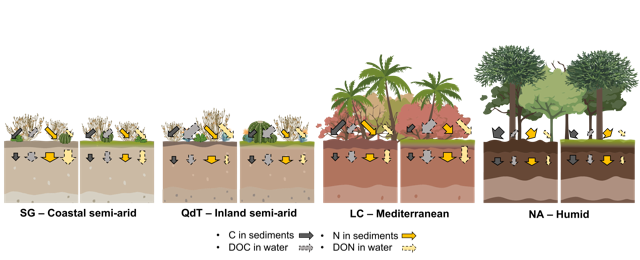
\includegraphics[width=1\textwidth]{img/M2-Figure_4.png}
	\caption{Total carbon (C) and nitrogen (N) fluxes in sediment and water for the four study sites. Diagonal arrows represent surface runoff. Arrows pointing vertically downward represent percolation. The diagrams on the right, with a light green surface, represent the BSC+ treatments, and the one on the left represents the BSC- treatments. Grey-filled arrows correspond to C fluxes, and yellowish arrows to N. At the same time, arrows with solid borders correspond to fluxes attached to the sediments and dashed arrows correspond to fluxes dissolved in water. Each type of arrow is proportional within each group in width to the concentration of nutrients and in length to their mass.}
	\label{fig:M2-F4}
\end{figure}

\FloatBarrier

The increase in C/N ratio along the climatic gradient, from arid to humid conditions, indicates a shift in the dominant processes from mineralization to immobilization \citep{Brust2019}. This shift implies enhanced N recycling and increased stability of SOM in more humid environments \citep{Oeser2020}. However, the presence of biocrusts altered these patterns, where in SG and QdT there were no changes in the C/N of the bare soil. In LC and NA, however, the presence of biocrusts implied a reduction in the C/N of the sediments, suggesting that biocrust-influenced sediments contain less C but more N, which is often a limiting element for biological activity \citep{Hanrahan2005} and may pose a higher risk as a watercourse pollutant \citep{Dodds2016}.

The composition of the percolated sediments in the soil profile also varied with climate and the presence of biocrusts. The C\textsubscript{T} of the sediments followed the climatic gradient, increasing with moisture. Biocrust presence reduced C\textsubscript{T} in sediments compared to bare soil, suggesting that the sediments serve as a C source for the organisms in the biocrusts \citep{Sancho2016}. Thus, biocrusts reduce long-term C pools in the subsoil and concentrate C where there is more biological activity \citep{Baumert2021}. C\textsubscript{T} of sediments along the sites and biocrust conditions followed the same pattern as C\textsubscript{T} of soils published by \citet{RiverasMunoz2022}. The N\textsubscript{T} of sediments followed a similar climatic gradient as the C\textsubscript{T}, with a significant increase when moving to wetter conditions, reflecting the general pattern of net primary productivity \citep{LeBauer2008}. However, the effect of biocrust on N\textsubscript{T} in sediments mobilized by percolation was not significant per se but depended on the specific site. The above indicates a change in the effect of biocrusts on N\textsubscript{T} at the different sites, where the sediments act as a source of N in LC and NA but as a sink in SG and NA. These differences in the direction of N flux in the different environments had a direct effect on the C/N ratio, indicating rapid mineralization and release of N for plants in SG, QdT and LC and a state of equilibrium between mineralization and immobilization in NA \cite{Brust2019}. The lack of difference in the C/N ratio, together with a significant increase in the values of C\textsubscript{T} and N\textsubscript{T} when biocrusts are present, highlights biocrusts as active agents in the fixation of these elements but that maintain the equilibrium in the ratio of these elements when considering sediments mobilized by infiltration under different climatic conditions.

The liquid phase of both percolation and runoff showed changes in DOC and DON content in the presence of biocrusts, representing readily available organic C and N sources \citep{Bernal2005}. A meta-analysis by \citet{Xu2022} found that BSCs generally increased SOC by 70.9\% compared to uncrusted soil, with the strongest positive effects observed in deserts and with mixed crusts (containing multiple biocrust types). Biocrust removal significantly increased both DOC and C\textsubscript{T} mobilization, especially under high-intensity rainfall. For example, \citet{Chamizo2017} found that annual DOC mobilization could increase up to three-fold and C\textsubscript{T} mobilized in sediments up to ten-fold in biocrust-removed soils compared to soils with intact biocrusts, with the most pronounced effect during the first rainfall event after removal. Furthermore, \citet{Aanderud2018} found evidence for the initiation of fungal loops -- where fungi translocate resources between soils and plants -- in cyanobacteria-dominated crusts. Specifically, they showed that \ce{^{15}N} from \ce{^{15}NH4+} moved \SI{40}{\milli\metre\per\hour} in biocrust soils. This highlights the immediate impact of biocrust disturbance on C loss through water erosion, and the potential role of fungi in nutrient cycling. \citet{Young2022} significantly expand on that, demonstrating this availability varies greatly with biocrust successional stage. Lightly pigmented cyanobacterial crusts leached more dissolved nitrogen, while moss crusts released significantly more dissolved organic carbon. Although these differences did not immediately alter mineral soil microbial respiration, soil beneath moss crusts showed higher long-term \ce{CO2} flux, suggesting organic C accumulation. Thus, biocrust type crucially regulates nutrient and carbon fluxes to deeper soil, impacting dryland ecosystem function.

Our results suggest that organic C and N mobilization in water and sediments depends on the interplay of climatic conditions, site characteristics and biocrust presence, in agreement with \citet{Austin2004}. We observed that runoff models captured biocrust effects more accurately than infiltration models, probably because the influence of biocrusts is strongest at the surface and decreases with depth - beyond \SI{7}{\centi\meter} in our study. This observation is consistent with \citet{Williams2022}, who only consider biocrust effects to a depth of about {4}{\centi\meter} in runoff models. This confirms that the presence of surface biocrusts can influence nutrient mobilization in water and sediments \citep{Belnap2003,RodriguezCaballero2013}, not only in arid ecosystems.

Furthermore, our study found that sediment N loss was explained by site and biocrust, without interactions between the two factors, indicating that both site and biocrust have individual effects on N mobilization. The importance of biocrust suggests similar mechanisms in each site studied, where biocrusts act as a source of N that moves vertically and is relocated in depth by infiltration at the expense of DON in the runoff. In contrast, DOC loss in runoff was significantly explained by site, biocrust and their interaction, whereas percolation DOC was only influenced by site. These results suggest that DOC flux is controlled by complex interactions between the site and biocrust at the surface, which decrease with depth.

These results highlight the nuanced role of biocrust in regulating C and N source and sink dynamics, with effects varying significantly across climatic gradients and between surface and subsurface processes such as surface runoff and percolation. The effects of biocrust were particularly pronounced on surface-associated runoff dynamics, while their influence on subsurface and percolation fluxes diminished. These observations highlight the importance of considering local environmental conditions and biocrust interactions when assessing their ecological functions and contributions to nutrient cycling. Overall, nutrient fluxes in water and sediments appear to be influenced by a combination of several factors, including climate and biocrust (structure, composition and activity). Further studies may be required to fully understand the mechanisms driving these interactions and their implications for ecosystem processes.

\section{Conclusions}

In this study, we investigated the role of biocrusts in erosion, infiltration, and C and N fluxes across climatic gradient in the Chilean Coastal Range, encompassing coastal and inland semi-arid, Mediterranean, and humid conditions. Biocrusts were abundant, though limited by human disturbance.

Our findings partially support our first hypothesis, showing biocrusts consistently reduce soil erosion and enhance infiltration, regardless of climate. However, their impact on surface runoff initiation varied. Rough-surfaced, bryophyte-dominated biocrusts in humid environments delayed runoff, an effect less pronounced in drier climates with smoother biocrusts. While generally reducing runoff volume (e.g., QdT), biocrusts unexpectedly increased it in one Mediterranean site (LC). Biocrusts significantly reduced sediment discharge across all climates, most effectively in the inland semi-arid site. While not altering infiltration time, they increased cumulative infiltration and facilitated fine particle movement into deeper soil.

Our second hypothesis, proposing climate-specific feedbacks, is also supported. Biocrusts influenced sediment nutrient dynamics. In semi-arid sites (SG, QdT), they increased sediment C and N, a trend reversed in wetter sites (LC, NA), demonstrating a climate-dependent shift in their function as nutrient sources/sinks. Biocrusts enhanced percolation, deep sediment transport, and N fluxes at depth, while reducing C loss via infiltration.

They also affected dissolved C and N. Initial dissolved C and N losses decreased with increasing humidity. Biocrusts generally reduced C losses; for N, they acted primarily as a source, mobilized by infiltration. Interactions were strongest at the surface, decreasing with depth.
These findings highlight the context-dependent impacts of biocrusts, revealing complex interplay between biotic and abiotic factors. By protecting soil, modulating water infiltration, and interacting dynamically with nutrients, they are crucial ecological players in drylands and other ecosystems.

\section*{Acknowledgements}

This study results from several years of work and the successful completion of the field expedition, which was significantly delayed by the global pandemic. It would not have been possible without the collaboration and support of many individuals. In addition to the co-authors, we are deeply grateful to the following students for their invaluable contributions: Martin Loyola, Antonia Tertelmann, Hugo "el fenómeno" Pérez, Merle Eichholz, Rae Bischoff, Kerstin Rau, Daniella Verdugo, Bruno Araya, Sofia Vila, and Larissa Werner. We are grateful to the Chilean National Forest Corporation (CONAF) and Sucesión Gálvez Muñoz for providing access to the study sites. The study was funded by the German Science Foundation (DFG) SPP 1803 "EarthShape" (grant number SCHO 739/17-2). We acknowledge support by the Open Access Publishing Fund of the University of Tübingen.

\section*{Data availability}

Data is available on [Dryad](https://doi.org/10.5061/dryad.m0cfxppfm)

\section*{Declaration of generative AI and AI-assisted technologies in the writing process}

During the preparation of this work, the author(s) used ChatGPT3.5 and Grammarly in order to improve English language usage, grammar, clarity, and readability, as none of the authors is a native speaker. After using these tools/services, the author(s) reviewed and edited the content as needed and take(s) full responsibility for the content of the publication.

\bibliographystyle{natbib} % Consider changing to a style compatible with KOMA/natbib if issues arise
\bibliography{literatur_all_clean}